\chapter{Introduction to Calculus}

\section{Chapter Overview}
\begin{itemize}
    \item \textbf{Historical Context:} Mathematicians of the 17th century were keenly interested in studying motion
    \begin{itemize}
        \item Objects on or near Earth
        \item Motion of planets and stars
    \end{itemize}
    
    \item \textbf{Key Insights:} Motion study involved both speed and direction
    \begin{itemize}
        \item Direction at any instant: along the tangent line to the path
        \item Need for precise mathematical tools
    \end{itemize}
    
    \item \textbf{The Limit Concept:} Fundamental to finding
    \begin{itemize}
        \item Velocity of moving objects
        \item Tangent lines to curves
    \end{itemize}
    
    \item \textbf{Function Behavior:} Limits help us distinguish between
    \begin{itemize}
        \item Continuous variation (small changes in $x$ → small changes in $f(x)$)
        \item Discontinuous behavior (jumps, erratic variation)
        \item Unbounded growth or decay
    \end{itemize}
    
    \item \textbf{Our Approach:} Develop limits intuitively, then formally
\end{itemize}
\section{Slopes and Average Rate of Change}

% Slide: Motivation and Overview
\section{Motivation: Why Study Change?}
  \begin{itemize}
    \item Calculus explores how quantities change : how change in one quantity is related to a change in anotherand provides tools for modeling these changes.
    \item Functions link inputs ($x$) to outputs ($y=f(x)$); we investigate how $y$ varies as $x$ moves over an interval.
    \item Real-world example: Predicting economic indicators, modeling speeds, and more.
  \end{itemize}

% Slide: Defining Average Rate of Change
\section{Average Rate of Change and Secant Lines}
  \begin{block}{Definition}
    For a function $f(x)$ on interval $[x_{1},x_{2}]$, the \emph{average rate of change} over that interval is
    \[ 
      = \frac{\Delta y}{\Delta x} = \frac{f(x_{2})-f(x_{1})}{x_{2}-x_{1}} = \frac{f(x_{1}+h) - f(x_{1})}{h}, h \neq 0
    \]
    which geometrically represents the slope of the secant line between $(x_{1},f(x_{1}))$ and $(x_{2},f(x_{2}))$.
  \end{block}
  \begin{itemize}
    \item Rise: $f(x_{2})-f(x_{1})$
    \item Run: $x_{2}-x_{1}$
    \item The secant line smooths out fluctuations; its slope reports the net change per unit input over the interval.
    \item Approximating the curve over the interval with a straight line. 
  \end{itemize}

% Slide: Graphical Illustration
\section{Graphical Illustration}
  \begin{columns}
    \column{0.6\textwidth}
      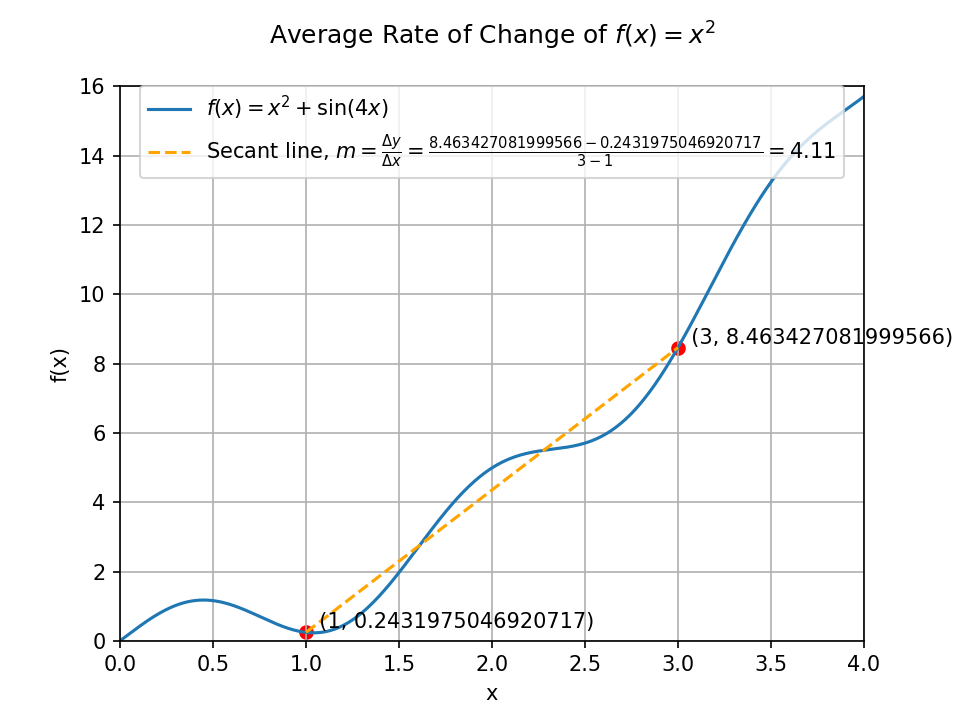
\includegraphics[width=\textwidth]{avg_rate_of_change.png}
    \column{0.4\textwidth}
      \begin{itemize}
        \item Focus on interval $[1,3]$ on the curve $y=f(x)$.
        \item Secant line (in orange) joins $(1,f(1))$ and $(3,f(3))$.
        \item Its slope measures the average change in $y$ per unit change in $x$.
      \end{itemize}
  \end{columns}

% Slide: Problem – Trivandrum to Chennai Average Speed
\section{Example: Trivandrum to Chennai Journey}
  \begin{columns}
    \column{0.5\textwidth}
      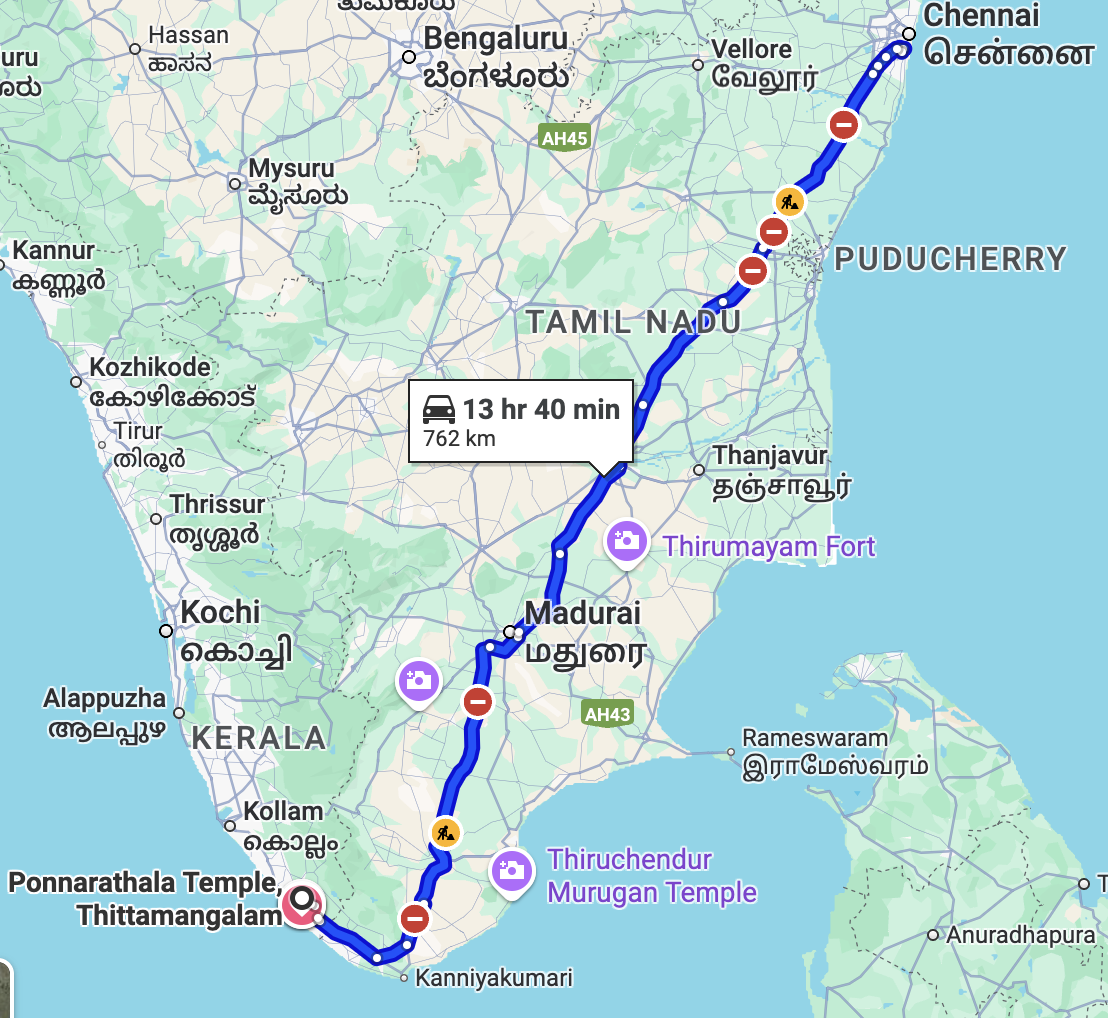
\includegraphics[width=\textwidth]{trivandrum_chennai_map.png}
    \column{0.5\textwidth}
      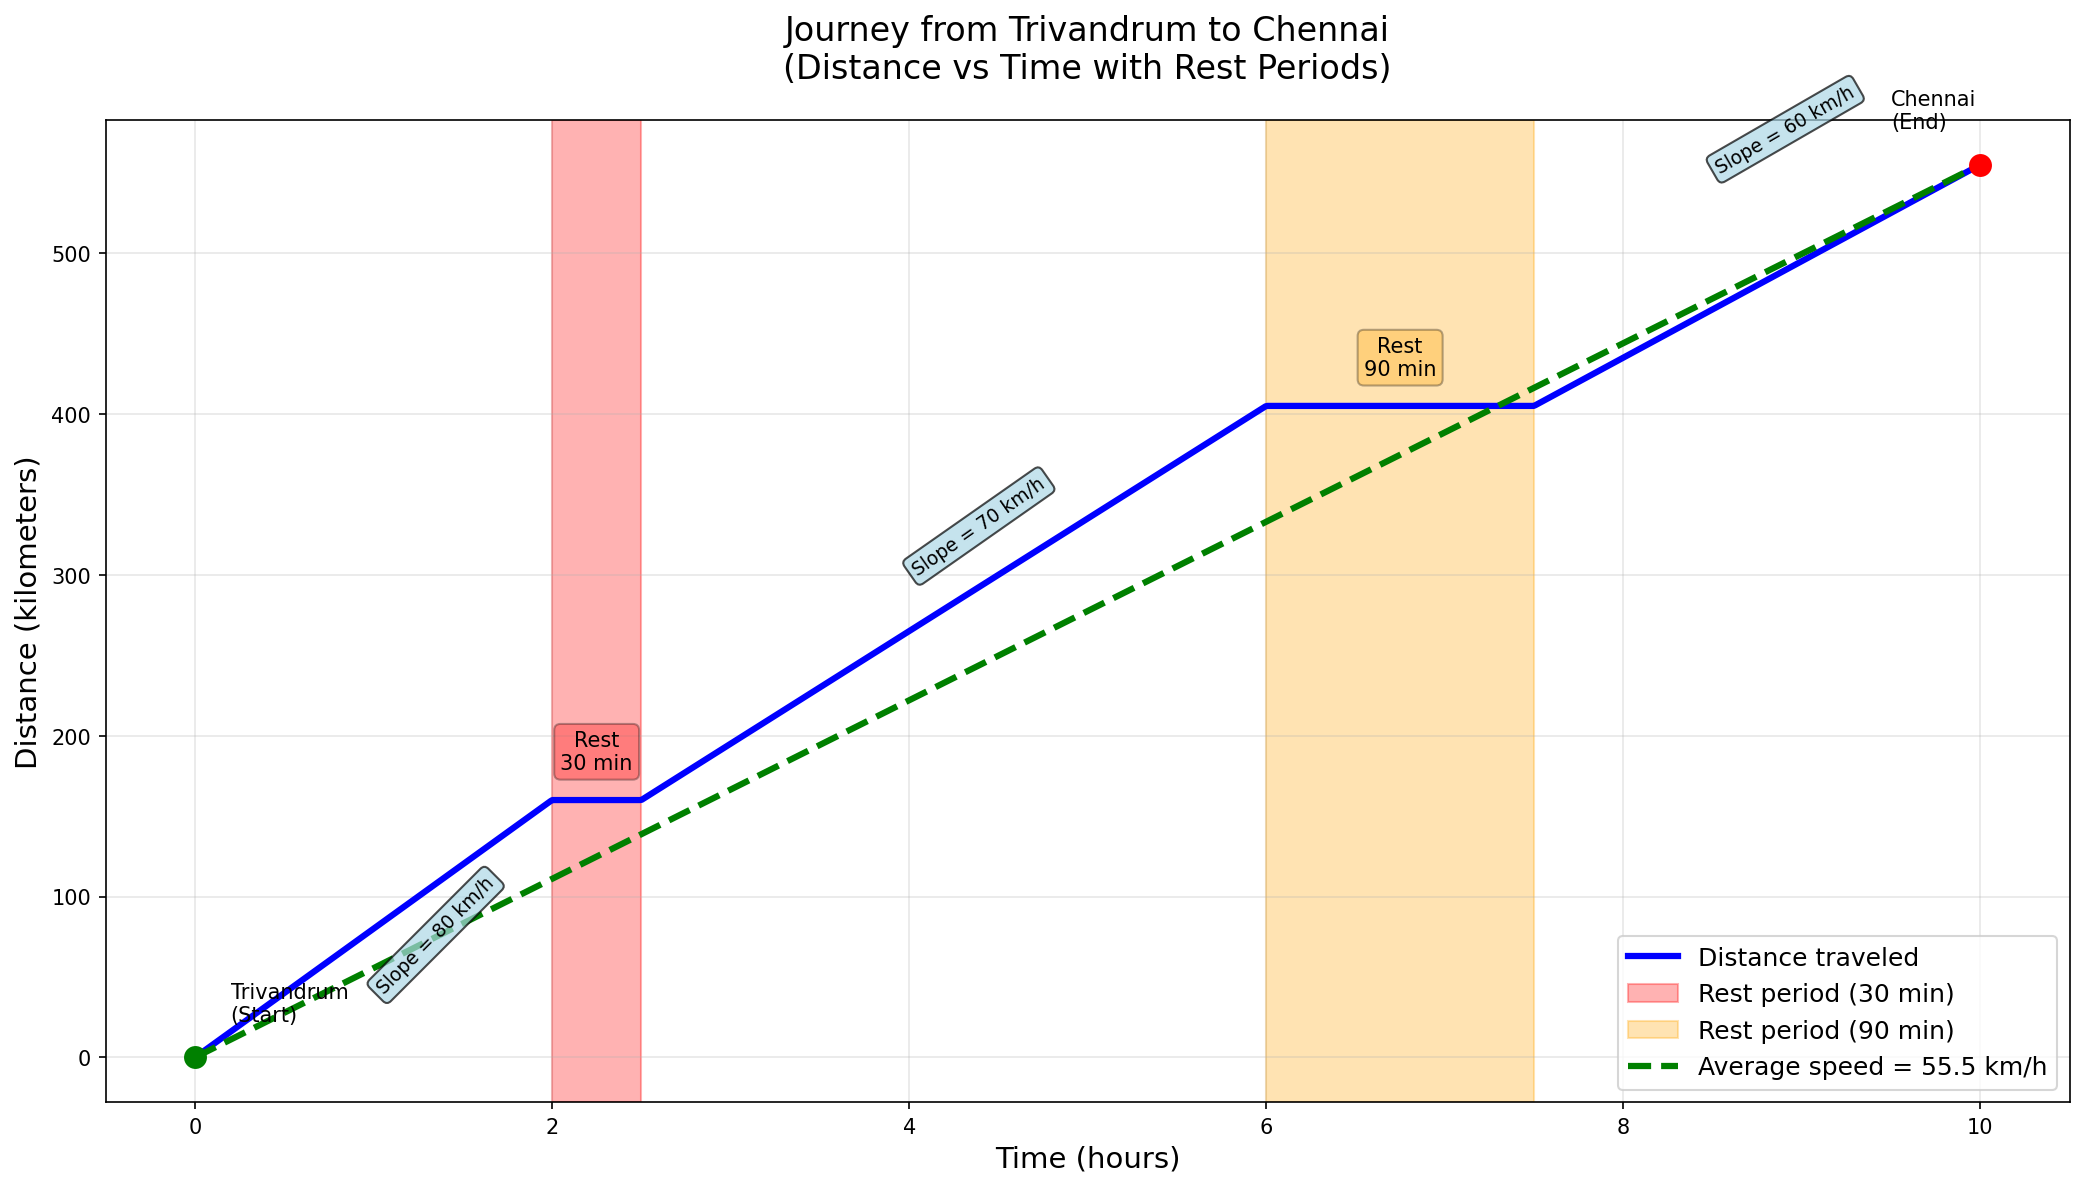
\includegraphics[width=\textwidth]{trivandrum_chennai_journey.png}
  \end{columns}
  \vspace{1ex}


  \begin{itemize}
    \item Total distance: 762 km
    \item Total time (including stops): 15 hours
    \item Average speed: $\dfrac{762}{15}\approx50.8$ km/h
  \end{itemize}
  \begin{solutionblock}
    Average speed $=\dfrac{h}$.  
  This illustrates how the secant slope over an interval gives overall performance even with rest periods.
  \end{solutionblock}

% Slide: Sensitivity to Rounding
\section{Rounding and Accuracy}
  \begin{columns}
    \column{0.58\textwidth}
      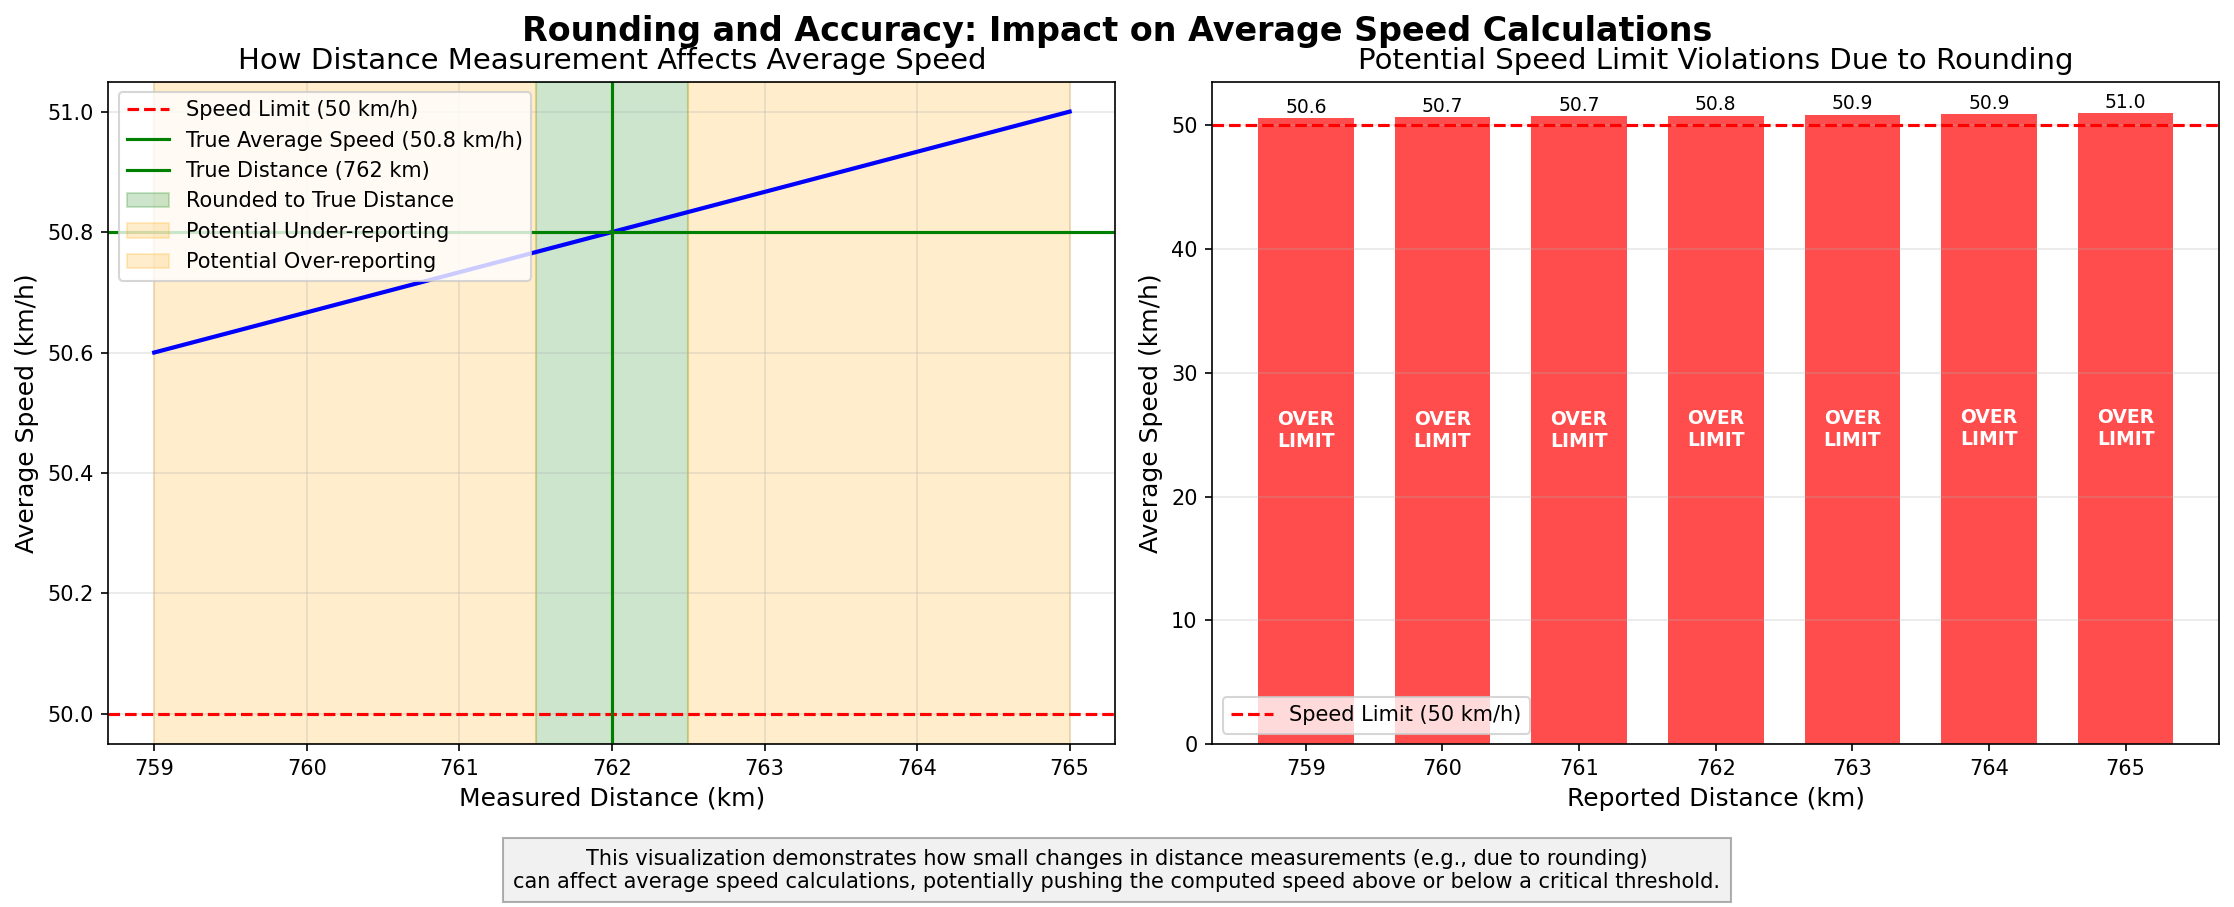
\includegraphics[width=\textwidth]{rounding_accuracy_demo.png}
    \column{0.42\textwidth}
      \begin{itemize}
        \item Distance measurements rounded to nearest kilometer introduce potential error
        \item For our journey: $\dfrac{762\text{ km}}{15\text{ h}} \approx 50.8$ km/h
        \item A mere 3 km error in measurement can push calculated speed above/below the 50 km/h limit
        \item Data precision is important.
      \end{itemize}
  \end{columns}

% Slide: Toward Instantaneous Rate of Change
\section{Instantaneous Rate of Change}
  \begin{itemize}
    \item Instantaneous speed corresponds to slope of tangent line at a point.
    \item As secant interval shrinks ($b\to a$), average rate approaches derivative $f'(x)$.
    \item Next: Formalize tangent lines and derivatives.
  \end{itemize}

\frametitle{Why Instantaneous Rate of Change?}
\begin{itemize}
  \item Average rate of change provides overall performance but lacks detail.
  \item Instantaneous rate of change captures behavior at a specific moment while average rate is over an interval
  \item Essential for understanding dynamic systems (e.g., velocity, acceleration).
  \item Instantaneous rate of change = calculate average rathe of change over smaller and smaller intervals.
\end{itemize}
\section{Secants to Tangents}
  \begin{block}{Problem}
    Find the slope of the tangent line to the parabola $y = x^{2}$ at $P(2,4)$ by looking at slopes of secant lines through $P$ and a nearby point $Q(2+h,(2+h)^{2})$ and letting $h \to 0$.
  \end{block}

  \begin{block}{Average rate of change (secant slope)}
    Between $x=2$ and $x=2+h$ (with $h \ne 0$):
    \[
      \text{slope}(h)=\frac{(2+h)^2 - 4}{h}
    \]
  \end{block}

  \begin{itemize}
    \item Expand: $(2+h)^2 = 4 + 4h + h^{2}$
      \[
        \text{slope}(h)=\frac{4+4h+h^{2}-4}{h}= \frac{4h+h^{2}}{h}
      \]
    \item Simplify (since $h \ne 0$): $\text{slope}(h)=4 + h$
    \item Sample values:
      \[
        h=1\!\to\!5,\; h=0.5\!\to\!4.5,\; h=0.1\!\to\!4.1,\; h=0.01\!\to\!4.01,\; h=-0.01\!\to\!3.99
      \]
    \item The secant slopes get closer to $4$ as $h$ gets closer to $0$.
    \item Limit viewpoint:
      \[
        \lim_{h\to 0} \frac{(2+h)^2 - 4}{h} = \lim_{h\to 0} (4 + h)=4
      \]
      So the instantaneous rate of change (slope of the tangent line) at $x=2$ is $4$.
  \end{itemize}



  \frametitle{The Mean Value Theorem}
  \begin{figure}
    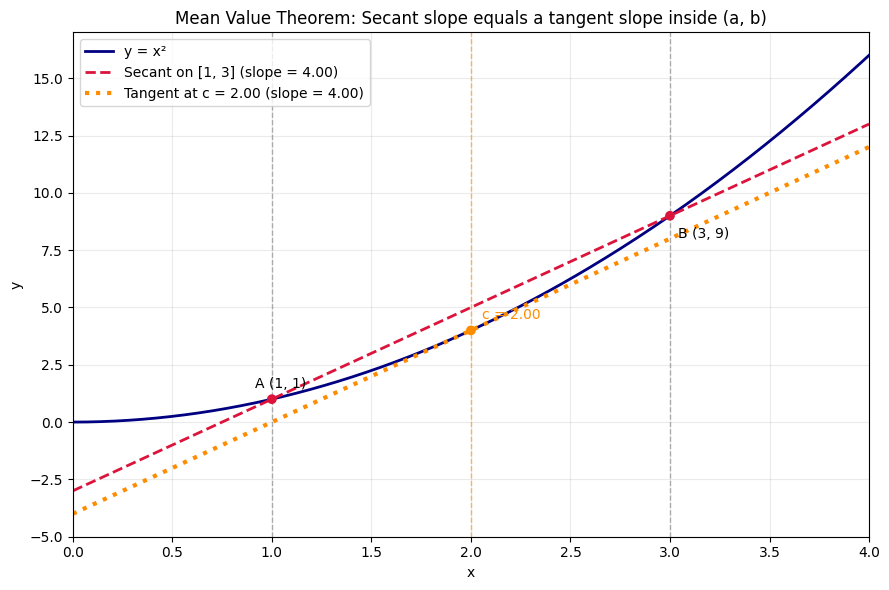
\includegraphics[width=0.75\textwidth]{mean_value.png}
    \caption{Mean Value Theorem: There exists a point $c$ where the tangent equals the secant.}
  \end{figure}
% Slide: Mean Value Theorem (informal, no derivatives)
\section{The Mean Value Theorem (informal, no derivatives)}
  \begin{block}{Statement}
  For a smooth curve $y=f(x)$ on an interval $[a,b]$, the \emph{average rate of change}
  \[ \dfrac{f(b)-f(a)}{b-a} \]
  is realized as the slope of a \emph{tangent line} at some point $x=c$ with $a<c<b$.
  In other words, the secant line joining $(a,f(a))$ and $(b,f(b))$ has the same slope as
  the tangent line to the curve at some point inside the interval.
  \end{block}
  \vspace{0.5em}
\section{Displacement, Velocity, and Acceleration}
\section{Displacement}
  \begin{block}{Definition}
    The displacement $x(t)$ at time $t$ measures position on the real line relative to an origin $0$, so positive values indicate one direction and negative values the opposite.
  \end{block}
  \begin{itemize}
    \item Independent variable: time $t$ (typically seconds).
    \item Dependent variable: displacement $x$.
    \item Choice of origin and direction provides a signed measure of position.
  \end{itemize}

\section{Velocity}
  \begin{block}{Definition}
    The velocity $v(t)$ is the instantaneous rate of change of displacement $x(t)$.
  \end{block}
  \begin{itemize}
    \item $v(t)>0$ (motion in the positive direction), $v(t)<0$ (negative direction), or $v(t)=0$.
    \item Speed is the magnitude of velocity: $\text{speed}=\lvert v(t)\rvert$.
    \item A speedometer displays instantaneous speed.
  \end{itemize}

\section{Acceleration}
  \begin{block}{Definition}
    The acceleration $a(t)$ is the instantaneous rate of change of velocity $v(t)$.
  \end{block}
  \begin{itemize}
    \item $a(t)$ may be positive, negative, or zero.
    \item The term “deceleration” is often used when $a(t)$ is negative and quoted as a positive number by convention.
  \end{itemize}

\section{Example: Cannonball Projectile}
  \begin{figure}
    \centering
    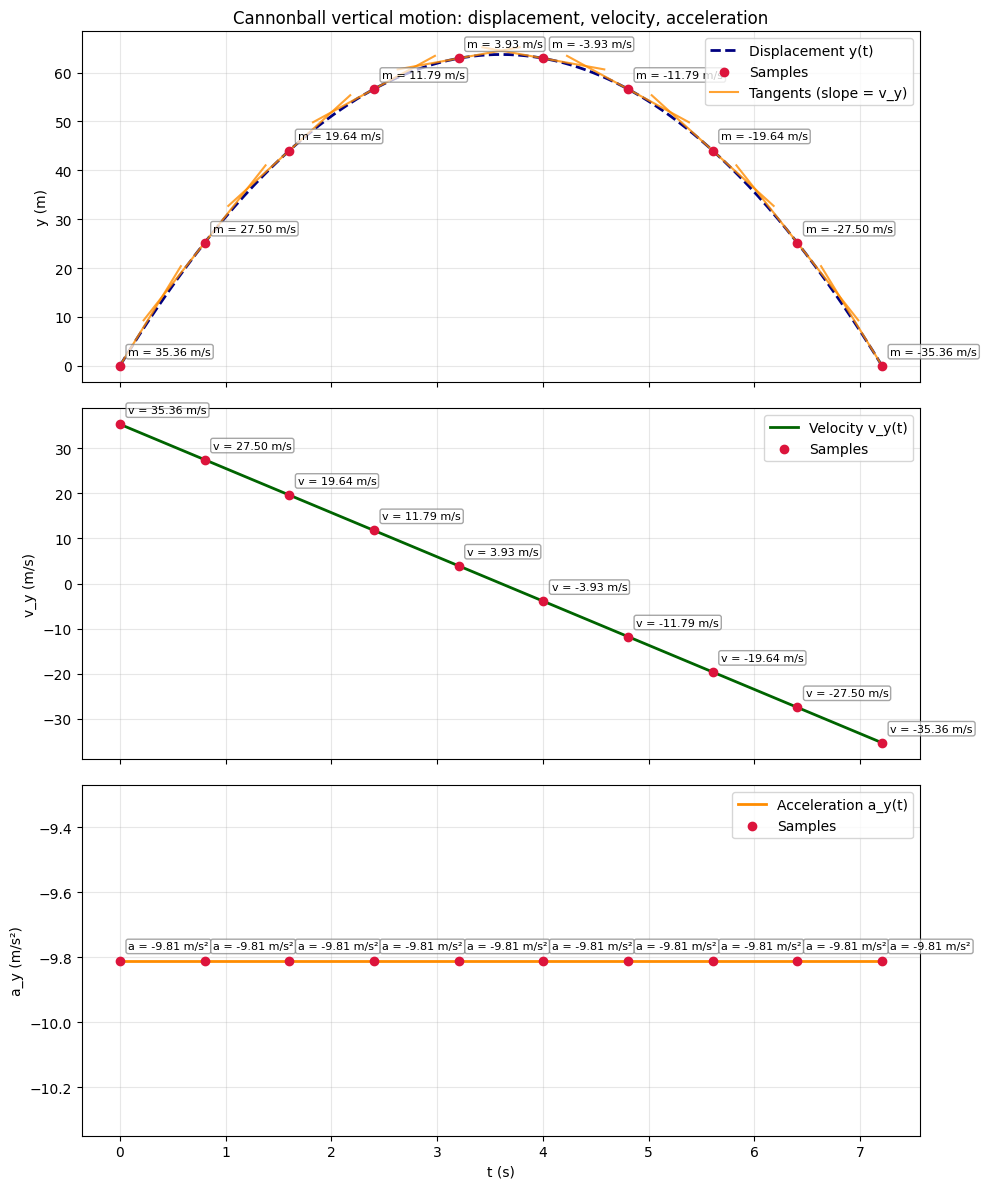
\includegraphics[width=0.5\textwidth]{cannonball.png}
  \end{figure}



